% \documentclass[a4paper, conference, compsoc]{IEEEtran}
\documentclass[12pt,a4paper]{article}
% \documentclass[%
%     pdftex,
%     oneside,			% Einseitiger Druck.
%     12pt,				% Schriftgroesse
%     parskip=half,		% Halbe Zeile Abstand zwischen Absätzen.
% %	topmargin = 10pt,	% Abstand Seitenrand (Std:1in) zu Kopfzeile [laut log: unused]
%     headheight = 12pt,	% Höhe der Kopfzeile
% %	headsep = 30pt,	% Abstand zwischen Kopfzeile und Text Body  [laut log: unused]
%     headsepline,		% Linie nach Kopfzeile.
%     footsepline,		% Linie vor Fusszeile.
%     footheight = 16pt,	% Höhe der Fusszeile
%     abstracton,		% Abstract Überschriften
%     DIV=calc,		% Satzspiegel berechnen
%     BCOR=8mm,		% Bindekorrektur links: 8mm
%     headinclude=false,	% Kopfzeile nicht in den Satzspiegel einbeziehen
%     footinclude=false,	% Fußzeile nicht in den Satzspiegel einbeziehen
%     listof=totoc,		% Abbildungs-/ Tabellenverzeichnis im Inhaltsverzeichnis darstellen
%     toc=bibliography,	% Literaturverzeichnis im Inhaltsverzeichnis darstellen
% ]{scrreprt}	% Koma-Script report-Klasse, fuer laengere Bachelorarbeiten alternativ auch: scrbook


% Basic packages
\usepackage[T1]{fontenc}
\usepackage[utf8]{inputenc}
\usepackage[scaled]{beramono}
\usepackage[english,ngerman]{babel,varioref}
\usepackage{xcolor}
\usepackage{amsmath}

% Tables
\usepackage{booktabs}
\usepackage{multirow}
\usepackage{longtable}
% Graphics and Includes
\usepackage[pdftex]{graphicx}
\graphicspath{{assets/img/}}
\DeclareGraphicsExtensions{.pdf,.jpeg,.png,.jpg}
\usepackage{tikz}
\usetikzlibrary{arrows.meta,bending,automata,shapes}
\usepackage[underline=true,rounded corners=false]{pgf-umlsd}

% Reduce distance before caption
\usepackage[skip=5pt]{caption}
% Bibliography
\usepackage[backend=biber, isbn=false, doi=false, style=ieee]{biblatex}
\addbibresource{bibliography.bib}
\AtBeginBibliography{\raggedright}
%\nocite{*}

% Gossar z.a. für acronyme
% \usepackage[acronym]{glossaries}
% \makeglossaries
\usepackage[printonlyused]{acronym} % falls gewünscht kann die Option footnote eingefügt werden, dann wird die Erklärung nicht inline sondern in einer Fußnote dargestellt

% \section*{Abkürzungsverzeichnis}
\begin{acronym}[AAAAAAA]
    \acro{wysiwyg}[WYSIWYG]{What you see is what you get}
\end{acronym}

% Colors
\definecolor{ListingBackground}{HTML}{E6E6E6}
\definecolor{LinkColor}{HTML}{000000}


% Font
\usepackage[onehalfspacing]{setspace}
\usepackage{lmodern}
\usepackage[official]{eurosym}
\usepackage{enumitem}
\usepackage[locale=DE]{siunitx} % SI Units für Währungen
\DeclareSIUnit{\EUR}{\text{\euro}} % Beispielverwendung: \SI{10.10}{\EUR}

\usepackage[autostyle=true,german=quotes]{csquotes}
\usepackage{url}
\newcommand{\code}[1]{\texttt{#1}}

% Additional Setup
\usepackage[unicode=true,hypertexnames=false,colorlinks=true,linkcolor=LinkColor,citecolor=LinkColor,urlcolor=LinkColor,pdftex]{hyperref}

% Trennung von URLs im Literaturverzeichnis (große Werte [> 10000] verhindern die Trennung)
\defcounter{biburlnumpenalty}{10} % Strafe für Trennung in URL nach Zahl
\defcounter{biburlucpenalty}{500}  % Strafe für Trennung in URL nach Großbuchstaben
\defcounter{biburllcpenalty}{500}  % Strafe für Trennung in URL nach Kleinbuchstaben
\interfootnotelinepenalty=10000 % prevent all footnotes from breaking over a page.

% Configs
\setcounter{tocdepth}{1} % Limit table of contents to subsection
\sisetup{detect-weight=true, detect-family=true} % SI Units shall detect font weight and family
\setlist[description]{style=nextline} % Break definitions of terms to a new line (used by \begin{description} \item[foo] bar \end{description})
\renewcommand*{\bibfont}{\small}

%Hurenkinder und Schusterjungen vermeiden
\clubpenalty = 10000
\widowpenalty = 10000
\displaywidowpenalty = 10000

% Quellcode
\usepackage{listings}
\usepackage{float}
\usepackage{textcomp}
\lstset{
    inputpath=assets/listings,
    language=Java,			% Standardsprache des Quellcodes
    numbers=left,			% Zeilennummern links
    stepnumber=1,			% Jede Zeile nummerieren.
    numbersep=5pt,			% 5pt Abstand zum Quellcode
    numberstyle=\tiny,		% Zeichengrösse 'tiny' für die Nummern.
    breaklines=true,		% Zeilen umbrechen wenn notwendig.
    breakautoindent=true,	% Nach dem Zeilenumbruch Zeile einrücken.
    postbreak=\space,		% Bei Leerzeichen umbrechen.
    tabsize=2,				% Tabulatorgrösse 2
    basicstyle=\ttfamily\footnotesize, % Nichtproportionale Schrift, klein für den Quellcode
    showspaces=false,		% Leerzeichen nicht anzeigen.
    showstringspaces=false,	% Leerzeichen auch in Strings ('') nicht anzeigen.
    extendedchars=true,		% Alle Zeichen vom Latin1 Zeichensatz anzeigen.
    captionpos=b,			% sets the caption-position to bottom
    backgroundcolor=\color{ListingBackground}, % Hintergrundfarbe des Quellcodes setzen.
    xleftmargin=0pt,		% Rand links
    xrightmargin=0pt,		% Rand rechts
    frame=single,			% Rahmen an
    frameround=ffff,
    rulecolor=\color{darkgray},	% Rahmenfarbe
    fillcolor=\color{ListingBackground},
    keywordstyle=\color[rgb]{0.133,0.133,0.6},
    commentstyle=\color[rgb]{0.133,0.545,0.133},
    stringstyle=\color[rgb]{0.627,0.126,0.941},
    float,
    upquote=true
}


\colorlet{punct}{red!60!black}
\definecolor{delim}{RGB}{20,105,176}
\colorlet{numb}{magenta!60!black}

\lstdefinelanguage{json}{
    string=[s]{"}{"},
    stringstyle=\color{numb},
    literate=
     *{0}{{{\color{numb}0}}}{1}
      {1}{{{\color{numb}1}}}{1}
      {2}{{{\color{numb}2}}}{1}
      {3}{{{\color{numb}3}}}{1}
      {4}{{{\color{numb}4}}}{1}
      {5}{{{\color{numb}5}}}{1}
      {6}{{{\color{numb}6}}}{1}
      {7}{{{\color{numb}7}}}{1}
      {8}{{{\color{numb}8}}}{1}
      {9}{{{\color{numb}9}}}{1}
      {:}{{{\color{punct}{:}}}}{1}
      {,}{{{\color{punct}{,}}}}{1}
      {\{}{{{\color{delim}{\{}}}}{1}
      {\}}{{{\color{delim}{\}}}}}{1}
      {[}{{{\color{delim}{[}}}}{1}
      {]}{{{\color{delim}{]}}}}{1}
}

\lstdefinelanguage{yaml}{
  identifierstyle=\color{delim},
  sensitive=false,
  comment=[l]{\#},
  commentstyle=\color{purple}\ttfamily,
  stringstyle=\color{numb},
  morestring=[b]',
  morestring=[b]"
}

\lstloadlanguages{Python,Java,bash}

\usepackage[german,onelanguage,linesnumbered,ruled]{algorithm2e}
% Styling Kommentar
\newcommand\mycommfont[1]{\color{gray}\ttfamily{#1}}
\SetCommentSty{mycommfont}

% Runde Klammern um Bedingungen
\SetKwIF{If}{ElseIf}{Else}{wenn~(}{)~dann}{sonst wenn}{dann}{Ende}
\SetKwFor{ForEach}{für jedes~(}{)~tue}{Ende}

%Eingabe und Ausgabe Texte
\SetKwInOut{Input}{Eingabe}
\SetKwInOut{Output}{Ausgabe}
% Useful tools
\usepackage{blindtext}
\usepackage{lipsum}
\usepackage[section]{placeins} % Prevent figures and tables to float to new section
\usepackage[obeyFinal,backgroundcolor=yellow,linecolor=black]{todonotes}


%Angaben zur Arbeit
\def\myTitel{Lösen des Konzertproblems mithilfe evolutionärer Algorithmen}
\def\myArbeit{Seminararbeit}
\def\myFach{Computational Intelligence}
\def\myDatum{\today}
\def\myBetreuer{Prof. Dr. Braun}
\def\myGutachter{Strenger Gutachter}
\def\myBearbeitungszeit{Lange}
\def\myAbgabeort{Heilbronn}

%Angaben zur Person
\def\myAutor{Lea Poletin}
\def\myDegree{Master Informatik}
\def\myInstitution{DHBW CAS, Bildungscampus 13, 74076 Heilbronn}
\def\myMatrikelnr{8514262}
\def\myKurs{TMINF17}
\def\myFirma{SAP SE}
\def\myFirmenort{Walldorf}
%\section*{Abkürzungsverzeichnis}
\begin{acronym}[AAAAAAA]
    \acro{wysiwyg}[WYSIWYG]{What you see is what you get}
\end{acronym}

\begin{document}


\title{\myTitel}
\author{\myAutor~(\myMatrikelnr)\\
    \small{\myFach}\\
    \small{\myDegree}\\
    \small{\myInstitution}
}
\date{\myDatum}

\begin{titlepage}
	\begin{longtable}{p{8.2cm} p{5.4cm}}
		% Firmenlogo
		&
		
\includegraphics[width=5.4cm]{casLogo}
	\end{longtable}
	\addtocounter{table}{-1}
    {\let\newpage\relax\maketitle}
    \thispagestyle{empty}
    % \vfill
    \begin{abstract}
    \lipsum[66]
\end{abstract}
\end{titlepage}
% \begin{titlepage}
	\begin{longtable}{p{8.2cm} p{5.4cm}}
		% Firmenlogo
		&
		
\includegraphics[width=5.4cm]{casLogo}
	\end{longtable}
	\addtocounter{table}{-1}
	\enlargethispage{20mm}
	\begin{center}
		\vspace*{12mm}	{\LARGE\textbf \myTitel }\\
		\vspace*{12mm}	{\large\textbf \myArbeit}\\
		% \vspace*{12mm}	\langdeckblattabschlusshinleitung\\
		\vspace*{3mm}		{\textbf \myDegree}\\
		\vspace*{12mm}	des Studiengangs \myKurs\\
    \vspace*{3mm}		am DHBW CAS\\
		\vspace*{12mm}	von\\
		\vspace*{3mm}		{\large\textbf \myAutor}\\
		\vspace*{12mm}	\myDatum\\
	\end{center}
	\vfill
	\begin{spacing}{1.2}
	\begin{tabbing}
		mmmmmmmmmmmmmmmmmmmmmmmmmm             \= \kill
		\textbf{Bearbeitungszeit}       \>  \myBearbeitungszeit\\
		\textbf{Matrikelnummer, Kurs}  \>  \myMatrikelnr, \myKurs\\
		\textbf{Firma}                  \>  \myFirma, \myFirmenort\\
		\textbf{Betreuer}               \>  \myBetreuer\\
		\textbf{Gutachter}              \>  \myGutachter
	\end{tabbing}
	\end{spacing}
\end{titlepage}

\pagenumbering{Roman}

% Sperrvermerk
\thispagestyle{empty}
% Sperrvermerk direkt hinter Titelseite
\section*{Sperrvermerk}

\vspace*{2em}

Die vorliegende {\myArbeit} mit dem Titel {\itshape{} \myTitel{}\/}
enthält unternehmensinterne bzw. vertrauliche Informationen der {\myFirma},
ist deshalb mit einem Sperrvermerk versehen
und wird ausschließlich zu Prüfungszwecken am Studiengang
{\myDegree} der Dualen Hochschule Baden-Württemberg vorgelegt.
Sie ist ausschließlich zur Einsicht durch den zugeteilten Gutachter,
die Leitung des Studiengangs und ggf. den Prüfungsausschuss des Studiengangs
bestimmt.  Es ist untersagt,
\begin{itemize}
\item den Inhalt dieser Arbeit (einschließlich Daten, Abbildungen, Tabellen, Zeichnungen usw.) als Ganzes oder auszugsweise weiterzugeben,
\item Kopien oder Abschriften dieser Arbeit (einschließlich Daten, Abbildungen, Tabellen, Zeichnungen usw.) als Ganzes oder in Auszügen anzufertigen,
\item diese Arbeit zu veröffentlichen bzw. digital, elektronisch oder virtuell zur Verfügung zu stellen.
\end{itemize}
Jede anderweitige Einsichtnahme und Veröffentlichung – auch von Teilen der Arbeit – bedarf der vorherigen Zustimmung durch den Verfasser und {\myFirma}.

\vspace{3em}

\myAbgabeort, \myDatum
\vspace{4em}

\rule{6cm}{0.4pt}\\
\myAutor

\newpage

% Erklärung
\thispagestyle{empty}

\section*{Selbstständigkeitserklärung}
\vspace*{2em}


Ich versichere hiermit, dass ich meine {\myArbeit} mit dem Thema: {\itshape \myTitel } selbstständig verfasst und keine anderen als die angegebenen Quellen und Hilfsmittel benutzt habe. Ich versichere zudem, dass die eingereichte elektronische Fassung mit der gedruckten Fassung übereinstimmt.


\vspace{3em}
\noindent
\myAbgabeort, \myDatum
\\
\\
\noindent
\rule{6cm}{0.4pt}\\
\myAutor

\newpage


% \begin{abstract}
    \lipsum[66]
\end{abstract}
% \newpage

\pagestyle{plain}		% nur Seitenzahlen im Fuß

% Inhaltsverzeichnis
\begin{spacing}{1.1}
    \begingroup
        \pagestyle{empty}
        %für die Anzeige von Unterkapiteln im Inhaltsverzeichnis
        \setcounter{tocdepth}{2}

        \tableofcontents
        \clearpage
    \endgroup
\end{spacing}
\newpage

% Abkürzungsverzeichnis
\cleardoublepage
\section*{Abkürzungsverzeichnis}
\begin{acronym}[AAAAAAA]
    \acro{wysiwyg}[WYSIWYG]{What you see is what you get}
\end{acronym}


% Abbildungsverzeichnis
\cleardoublepage
\listoffigures

%Tabellenverzeichnis
\cleardoublepage
\listoftables

% Quellcodeverzeichnis
\cleardoublepage
\lstlistoflistings
\cleardoublepage

\pagenumbering{arabic}

\section{Einleitung}\label{sec:einleitung}
In einem kleinen Blasmusik Ensemble mit regelmäßigen Auftritten, kommt es immer wieder zu Diskussionen 
bezüglich der Setliste. Neben der Dauer des Musikstückes sind bei der Auswahl der Stücke einige 
weitere Eigenschaften zu beachten. Eines ist beispielsweise die Anstrengung für die einzelnen Register(Hochblech, Tiefblech und Holz). 
Besonders bei langen Auftritten, ist es wichtig nicht zu viele Stücke auszuwählen, die 
für einzelne Register besonders anstrengend sind. Die Anstrengung soll für alle Register ausgeglichen sein.
\subsection{Beschreibung des Problems}
 Dieser Programmentwurf, stellt die Basis für ein System dar, dass anhand verschiedener Kriterien eine 
 Auswahl von Stücken zusammenstellt, die möglichst die Kriterien \emph{Schwierigkeit, Bekanntheit, Stimmung} optimiert und dabei die 
 geforderte Auftrittszeit möglichst nicht unterschreitet oder überzieht. Die Kriterien werden in \autoref{sec:fitness} genauer 
 beschrieben.\\
 Diese Problemstellung lehnt somit an das \textit{Knappsack-Problem} an, 
 da der Fokus auf der Auswahl der Stücke liegt und nicht auf der Reihenfolge.
 Die Theoretischen Grundlagen wurden aus den Vorlesungsmaterialien, Folien und Beispiele, und zusätzlich
aus \cite{keller:2000} erarbeitet.
\subsection{Kurze Beschreibung des Ensembles}
Das Ensemble besteht aus: 
\begin{itemize}
    \item 2 Trompeten (Hochblech)
    \item 2 Saxophone (Holzbläser)
    \item 1 Posaune (Tiefblech)
    \item 1 Tuba (Tiefblech)
    \item 1 Schlagzeug 
\end{itemize} 

Für einen Auftritt stehen 73 Stücke zur Auswahl, die zusammengestellt werden können. Dabei ist zu erwähnen, dass alle Stücke bei einem Auftritt gespielt werden können, 
da die Stücke bereits für die hinsichtlich der Auftrittsart (Stimmungsauftritt) angepasst sind. 
Die Auftritte haben eine Dauer von 120 Minuten.
\input{content/02_Liedeigenschaften}
\section{Genotyp und Phenotyp}\label{sec:genotypPhenotyp}
\subsection{Genotyp}
Der Genotyp ist ein Bitstring, der Beschreibt welche Lieder gespielt werden und welche nicht.
Dabei steht die 1 dafür, dass ein Lied ausgewählt wurde und besitzt so die Form

\begin{equation}
    \label{eqn:genotyp}
    \begin{split}
        x_i &\in \{ 0,1 \} \\
        x_i &= 1 \Rightarrow \text{Stück $i$ wird in die Setliste aufgenommen} \\
        x   &= x_1x_2...x_n \in \{0,1\}^n\text{ mit $n = $ Anzahl der gespielten Stücke}
    \end{split}
\end{equation}

\subsection{Phenotyp}
Der Phenotyp ist die Setliste mit allen Liederobjekten und wird für die
Berechnung der Fitness verwendet.
Er besitzt neben der Stückbezeichnung alle weiteren in \autoref{sec:settings}
beschriebenen Eigenschaften. \autoref{lst:phenotyp} zeigt die Implementierung der Klasse
eines Phenotyps.

\lstinputlisting[
    float,
    floatplacement=H,
    caption=Klasse für einen Phenotyp,
    label=lst:phenotyp
]{phenotyp.java}

\subsection{Population}
\section{Bewertung}\label{sec:fitness}
Die Fitnessfunktion soll die so auswählen, dass:
\begin{itemize}
    \item Die Dauer $d$ der Stücke möglichst genau der Auftrittszeit 120 Minuten entspricht.
    \item Die allgemeine Schwierigkeit $s$ möglichst minimiert wird. Hierbei ist zu erwähnen, dass die hier
        angegebene Schwierigkeit nicht zwingend der Durchschnitt der Registerschwierigkeiten darstellt, denn
        beispielsweise im Bezug auf das Zusammenspiel kann die allgemeine Schwierigkeit höher sein.
    \item Die Stimmung $m$ und die Bekanntheit $n$ möglichst maximiert wird.
    \item Die Schwierigkeit für Hochblech $s_{hoch}$, Tiefblech $s_{tief}$ und Holzblasinstrumente $s_{holz}$ möglichst ausgeglichen ist.
\end{itemize}
Um die Fitness des Phenotyps zu brechnen, müssen zunächst einige Basiswerte berechnet werden.
Für die allgemeine Schwierigkeit sowie für die Schwierigkeiten der einzelnen Register, zeigt dies \autoref{eqn:basis}. Hierbei werden alle Werte des
Phenotyps addiert. Durch den Bruch werden die Werte zusätzlich auf einen Wert zwischen $0$ une $1$ normiert.
Die Formeln für $m(x)$ und $n(x)$ sind identisch.
\begin{equation}
    s(x) = \frac{\sum_{i=0}^{n} x_i * (10 - s(i)) }{n * 10}
    \label{eqn:basis}
\end{equation}

Die Dauer sollte möglichst der geforderten Auftrittszeit entsprechen. Wird die Auftrittszeit nicht erfüllt
oder überschritten, soll sich dies negativ auf die Fitness des Phenotyps auswirken. Aus diesem Grund wird das
Ergebnis in \autoref{eqn:penalty} negiert. Auch in dieser Formel werden zunächst alle Differenzen zur geforderten
Spielzeit addiert. Die Bildung des Quadrats sorgt dafür, dass sowohl unterschreiten wie auch überschreiten
positive Werte ergibt.
Auch in \autoref{eqn:penalty} sorgt der Bruch für eine Normierung der Werte.

\begin{equation}
    penalty(x) = -\left( \frac{\sum_{i=0}^{n}x_i * (d(i)-120)}{120}\right)^2
    \label{eqn:penalty}
\end{equation}

Um einen Wert für die faire Verteilung der Schwierigkeit zu berechnen ist es zunächst notwendig, den Durchschnitt der
Schwierigkeit der Register zu berechnen. Dies zeigt \autoref{enq:avg}

\begin{equation}
    avg(x) = \frac{s(x)_{hoch} + s(x)_{tief} + s(x)_{holz}}{3}
    \label{enq:avg}
\end{equation}

Anschließend kann dieser Wert verwendet werden, um, wie in \autoref{eqn:fair} dargestellt,
den mittleren quadratischen Fehler zu berechnen.
\begin{equation}
    g(x) = \frac{((avg(x) - s(x)_{hoch}) + (avg(x) - s(x)_{tief}) +(avg(x) - s(x)_{holz}))^2}{3}
    \label{eqn:fair}
\end{equation}

Durch die Vorberechnung der einzelnen Werte ist die eigentliche Fitnessfunktion stark reduziert.
\autoref{eqn:fitness} zeigt die Fitnessfunktion mit allen zuvor beschriebenen Kriterien.
\begin{equation}
    f(x) = w_p * p(x) + w_s * s(x) + w_m * m(x) + w_n * n(x) +  w_g * g(x)
    \label{eqn:fitness}
\end{equation}

% \lstinputlisting[
%     float,
%     floatplacement=H,
%     caption=Implementierung der Fitnessfunktion,
%     label=lst:fitness
% ]{fitness.java}
\section{Kombination}\label{sec:eltern}
Da der Genstring in diesem Konzertproblem sehr lange ist, 73 Elemente, bietet es sich an einen Multi-Point-Crossover zu verwenden.
Dabei werden die beiden Eltern an $n$ zufällig gewählten Stellen getrennt und auf zwei neue Genstrings aufgeteilt.
\autoref{img:multiCrossover} zeigt anschaulich wie ein 3-Point-Crossover funktioniert. An je mehr Punkten
der Genstring geteilt und wieder zusammengesetz wird desto einen großeren Unterschied besitzen die Kinder von
den Eltern. Das Crossover an 3 Punkten bietet sich in dieser Anwendung an, da so der Unterschied nicht zu groß aber auch nicht zu klein ist.

\begin{figure}[h]
    \begin{minipage}{\textwidth}
	    \centering
        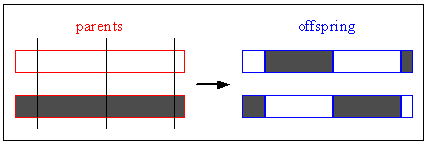
\includegraphics{multiPointCrossover.PNG}
	    \caption{Multi-Point-Crossover {http://www.geatbx.com}}
        \label{img:multiCrossover}
    \end{minipage}
\end{figure}

\section{Selektion}
Für die Selektion der Eltern bietet sich die Tournament Selection an.
Diese wählt zufällig mehrere Chromosome aus und selektiert das Chromosom mit der besten Fitness. Das Verfahren der
Tournament Selection ist in \autoref{img:tournament} dargestellt.


\begin{figure}
    \begin{minipage}{\textwidth}
        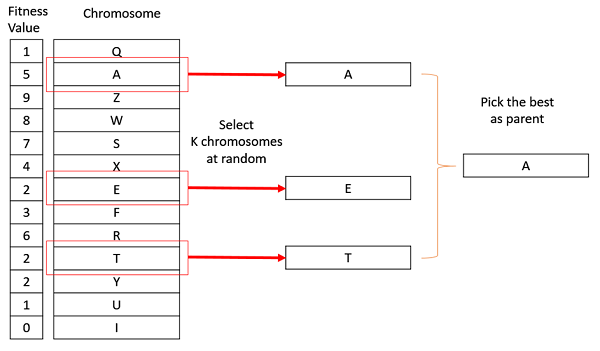
\includegraphics[width=\textwidth]{tournament_selection.jpg}
        \caption{Tournament Selection {https://www.tutorialspoint.com}}
        \label{img:tournament}
    \end{minipage}
\end{figure}

Da eine Population etwa 25 Gene besitzt, sollten für die Tournament Selection nicht mehr als 4 Chromosome zufällig gewählt werden.
Würden zu viele Chromosome gewählt werden, könnten auch einfach die besten zwei Gene der Population ausgewählt werden.
Dies würde zu wenig Veränderung der Gene führen und könnte dafür sorgen, dass nicht das globale sondern
lediglich ein lokales Optimum gefunden wird.

Ein Ansatz der genauer untersucht werden sollte ist es, an einem Zeitpunkt gegen Ende der
Evolution die Tournament Selection mit einer Zufall-Selektion auszutauschen.
Dies hat den Grund, dass zu diesem Zeitpunkt angenommen werden kann, dass alle
Gene eine ähnliche Fitness besitzen. Diese Idee könnte zu einer Optimierung der Selektion führen, dies 
müsste allerdings in einem Prototypen analysiert werden. 
\section{Mutationen}\label{sec:mutation}
Um neue Lösungen zu finden, werden die Eltern nicht nur kombiniert sondern auch zu
einer gewissen Wahrscheinlichkeit mutiert. Doch nicht jede Mutation ist für das Konzertproblem 
sinnvoll. 
\subsection{Analyse und Beschreibung verschiedener Mutationen}
\paragraph{Flip}
Bei dieser Mutation wird der Wert eines Bits verändert. Auf dieses Problem bezogen, 
bedeutet dies, dass ein Stück in die Setliste mit aufgenommen oder aus 
der Setliste gestrichen wird. 
\begin{enumerate}
    \item Entfernen eines Stückes: 
    \begin{itemize}
        \item Die Dauer des Auftritts wird kürzer, dies hat sehr wahrscheinlich eine Bestrafung und 
            damit eine Reduzierung der Fitness zur Folge. 
        \item Die Schwierigkeiten $s, s_{hoch}$, $ s_{tief}$ und $s_{holz}$ sinken ebenso. Dies sorgt allerdings 
            zu einer Steigerung der Fitness. 
    \end{itemize}
    \item Hinzufügen eines Stückes:
    \begin{itemize}
        \item Die Dauer des Auftritts wird länger, auch dies hat eine Reduzierung der Fitness zu Folge.
        \item Die Schwierigkeiten $s, s_{hoch}$, $ s_{tief}$ und $s_{holz}$ steigen ebenso, was auch zur Reduzierung 
            der Fitness führt. 
    \end{itemize}
\end{enumerate}
Dies bedeutet, dass die Fitness nach einem Flip nur steigen kann, wenn ein kurzes aber schwieriges Stück aus 
der Setliste entfernt wird. Allerdings könnte eine zunächst schlechtere Fitness den Algorithmus aus 
einem lokalen Optimum befreien.

\paragraph{Swap}
Beim Swap werden die Positionen von zwei Bits vertauscht. 
Daraus ergeben sich folgende Möglichkeiten für das Konzertproblem. 
\begin{enumerate}
    \item Fall \{$1 \longleftrightarrow 1$\}: Beide Stücke verbleiben in der Setliste.
    \item Fall \{$0 \longleftrightarrow 1$\} : Ein Stück wird von der Setliste gestrichen, dafür wird ein anderes Stück aufgenommen.
    \item Fall \{$0 \longleftrightarrow 0$\} : Beide Stücke sind nicht auf der Setliste.
\end{enumerate}

Fall 1 und Fall 3 sorgen weder für eine Verschlechterung noch zu einer Verbesserung. Dennoch sollten diese 
Fälle vermieden werden, da keine echte Mutation stattfindet. \\
Denkbar wäre es die zufällige Wahl der beiden Bits zu manipulieren. Das erste Bit wird aus der Menge der 
von der Setliste ausgeschlossenen Stücke gewählt und das zweite Bit aus der Menge der Setliste. 
Somit würde gewährleistet werden, dass bei jeder Swap-Mutation eine echte Mutation stattfindet. 
Der Austausch eines Stückes auf der Setliste mit einem anderen, ist für das Konzertproblem sehr sinnvoll, 
da die Dauer nur um die Differenz der Stückdauer verändert wird und nicht wie im Fall eines Flips um die gesamte
Länge eines Stückes. \\
Der Algorithmus hat durch den Swap die Möglichkeit die Population zu verbessern oder zu verschlechtern. 
Beide Fälle können sich positiv auf die Fitness des Endergebnisses auswirken. Aus diesem Grund 
wird der Swap für das Konzertproblem sinnvoll eingesetzt. 

\paragraph{Shuffel}
Beim Shuffel werden alle Werte neu vermischt, daher sorgt auch der Shuffel für eine gleichbleibende Anzahl an Stücken.
Der Unterschied zum \emph{Swap} ist der Umfang. Es wird nicht nur ein Stück ausgetauscht, sondern sehr viele. 
Das bedeutet, dass diese Mutation eine starke Änderung des Genotyps zur Folge hat. \\

Alle drei Mutationen haben ihre Berechtigung zur Lösung des Konzertproblems. Allerdings sollte 
der Flip nicht so oft sattfinden wie der Swap, da dieser die Fitness positiver beeinflusst. 
Dies kann mit hilfe von Wahrscheinlichkeiten erreicht werden. Eine Zufallszahl kann die Wahrscheinlichkeit 
für das Stattfinden einer Mutation bestimmen. 
Als initiale Einstellung könnten die Wahrscheinlichkeiten wie folgt gewählt werden: 
\begin{enumerate}
    \item $50\%$: Swap
    \item $25\%$: keine Mutation
    \item $20\%$: Shuffel
    \item $5\%$: Flip
\end{enumerate}
Diese Rangordnung sorgt dafür, dass die wahrscheinlichste Mutation ein Swap ist und ein Flip eher selten ausgeführt wird.

% \section{Optimierung}\label{sec:optimierung}
\subsection{Mehrzieloptimierung}
In der Zielfunktion müssen die vielen verschiedenen Eigenschaften gewichtet werden. 
Dies kann sehr kompliziert werden. Eine mögliche Optimierung für diese Problem ist die 
Verwendung eines Optimierers.


\section{Population und Evolution}\label{sec:popEv}
\subsection{Initialisierung der Population}
Die Initialisierung der Population kann entweder zufällig oder anhand von bereits vorhandenem Wissen.
In der Regel bietet es sich nicht an, die kompletete Population anhand von Wissen aufzubauen, da so
wenig neue Lösungen gefunden werden.\\
Dennoch wäre es in dieser Anwendung möglich einige vorhandene Setlisten in die Population einzustreuen und den Rest
anschließend mit zufälligen Werten zu füllen.

\subsection{Populationsgröße}
Die Populationsgröße sollte weder zu hoch noch zu niedrig sein. Typischer weiße werden Werte zwischen
20 und 30 gewählt. Diese kann später via \textit{Trial-and-Error} optimiert werden.

\subsection{Übersicht über den Algorithmus und die Evolution}

\begin{itemize}
    \item Zunächst wird die Population initialisiert.
    \item Anschließend wird die Fitness der einzelnen Chromosome anhand der in \autoref{sec:fitness} beschriebenen
        Formeln berechnet.
    \item Die Gene werden mithilfe der in \autoref{sec:eltern} beschriebenen Algorithmen selektiert und anschließend
        kombiniert.
    \item Nach der Kombination folgt die Mutation, die zufällig eine der in \autoref{sec:mutation} vorgestellten
    Mutationen auswählt.
    \item Der gesamte Algorithmus endet, die Abbruchbedingung siehe \autoref{subsec:Abbruchbedingung} erfüllt ist.
\end{itemize}

\subsection{Abbruchbedingung}\label{subsec:Abbruchbedingung}
Damit der Algorithmus irgendwan endet muss eine Abbruchbedingung definiert werden.
Hierzu gibt es verschiedene Möglichkeiten die auch kombiniert werden können:
\begin{itemize}
    \item Abbruch, falls in den letzen $n$ Wiederholungen keine Verbesserung stattfand.
    \item Abbruch, falls $n$ Wiederholungen beendet wurden.
    \item Abbruch, falls ein bestimmter Zielwert erreicht wurde.
\end{itemize}

\autoref{lst:abbruch} zeit die Java-Implementierung einer Abbruchfunktion die alle Drei Möglichkeiten
kombiniert. Die Maximale Anzahl an Wiederholungen wird durch die \textit{For-Schleife} eingehalten.
Die beiden anderen Bedingungen werden innerhalb der Schleife überprüft.
\lstinputlisting[
    float = h,
    floatplacement=H,
    caption=Abbruchfunktion,
    label=lst:abbruch
]{abbruch.java}
\section{Fazit und Ausblick}\label{sec:fazit}
Dieser Programmentwurf ist das Konzept für das Konzertproblem, welches 
eine Setliste für einen Auftritt erstellt und dabei die Dauer und die Schwierigkeit 
aber auch die Stimmung und den Bekanntheitsgrad der Stücke beachtet. 
Die Konzepte und Strategien müssen hierbei jedoch noch praktisch getestet und 
gegebenenfalls angepasst werden. \\
Aufbauend auf diesem Konzept wäre es denkbar mithilfe einer Permutations-Repräsentation 
auch die Reihenfolge der Stücke zu optimieren. Dies wäre dem Traveling Salseman Problem
ähnlich. Jedoch müsste hierbei nicht die Strecke der Orte minimiert werden, sondern es müssten 
viele andere Faktoren berücksichtigen. Ein Auftritt ist immer in einer ähnlichen Form 
aufgebaut.
\begin{enumerate}
    \item Das Einleitungsstück sollte nicht zu schwierig sein, aber dennoch die Aufmerksamkeit 
        des Publikums fangen.
    \item möglichst unterschiedliche Stücke, das heißt nach einigen schnellen Stücken vielleicht ein 
        langsames etc. 
    \item Gegen Ende des Auftritt einige Stimmungslieder bzw. Lieder mit hohem Bekanntheitsgrad
    \item Eine stimmungsvolle Zugabe und anschließend eine ruhige Zugabe. 
    \item Zum Abschluss muss, zumindest bei den Auftritten in Baden-Württemberg, das Badnerlied gespielt werden. 
\end{enumerate}

Dieser Grobablauf, könnte als Schablone für das Optimierungsproblem dienen. Die Stücke erhalten Eigenschaften, 
wie zum Beispiel \textit{mögliches Einleitungsstück} anhand derer über die Fitness entschieden wird. 



%\printacronyms{}
\printbibliography{}
\end{document}
